\chapter{Results and discussion}
To couple a surrogate model with optimizer, the model needs to be accurate enough. The \% error should be less than 2\% as suggested by \cite{alam2017thesis}. But Table \ref{Accuracy of different surrogate models} shows that even the best model is having average percentage error of 10 \% . The reason for this is due to the fact that we have less number of design points. We need more design points because pressure drag is highly depends on the frontal area exposed to the flow. Given a fixed volume, bodies with non-axisymmetric shapes will have higher frontal area compared to axisymmetric body as shown in fig.\ref{visual comparison}. This makes the non-axisymmetric body more 'bluffy'. This leads to flow separation which is a non-linear phenomenon. To fit a model which captures this non-linear phenomenon, the number of design points should be very much higher. 

\begin{figure}[H]
	\centering
	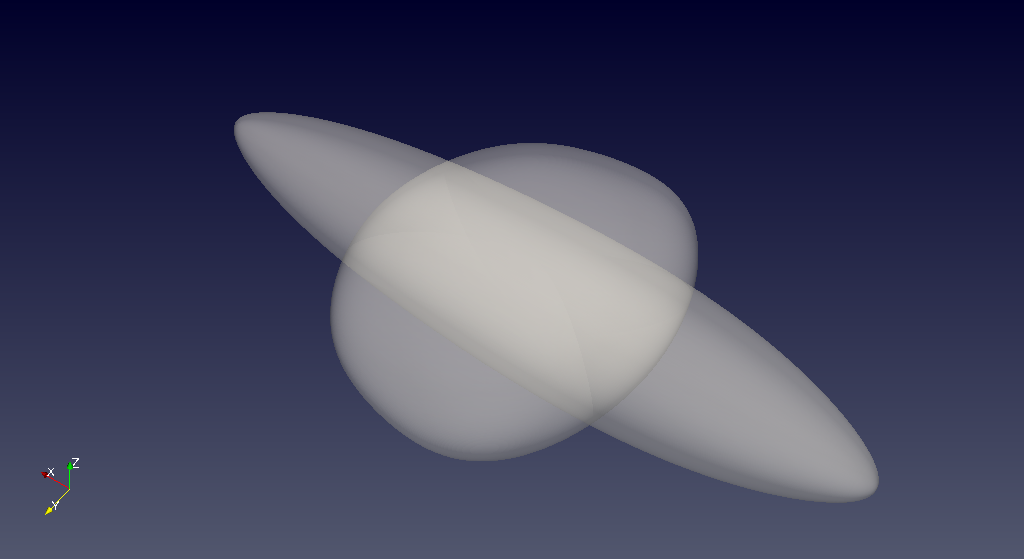
\includegraphics[width=300 pt]{rnd/visual_low_high.png}
	\caption{Visual comparison of low and high drag bodies}
	\label{visual comparison} %      only if needed
\end{figure}

The surface streamlines have been plotted in Figure \ref{low drag body} and \ref{high drag body}. It can be seen that long sleek body is having very less flow separation at the leading edge whereas the other body with more frontal area is have more flow separation and wake region.

\begin{figure}[H]
	\centering
	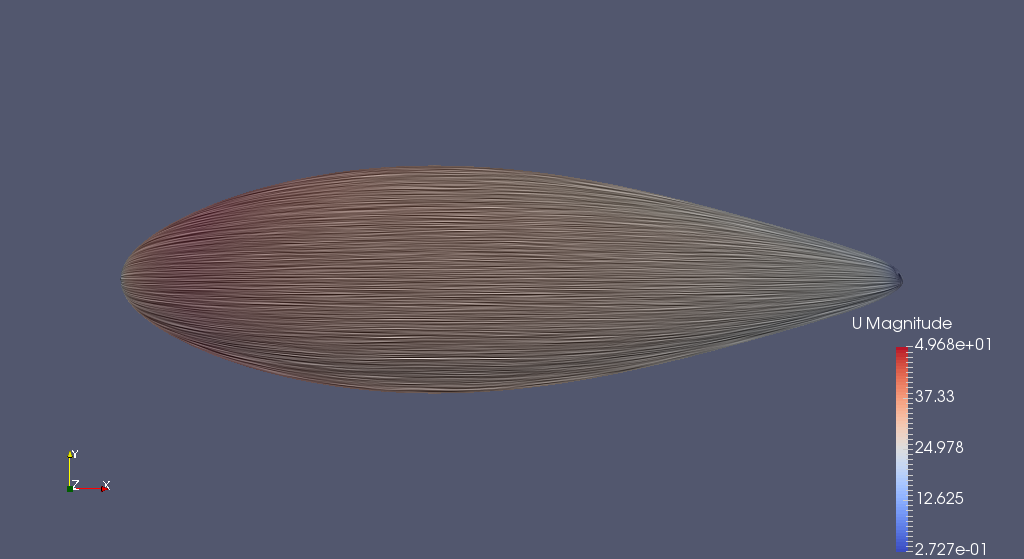
\includegraphics[width=300 pt]{rnd/streamlines_25_l.png}
	\caption{Surface streamlines on the body with low pressure drag}
	\label{low drag body} %      only if needed
\end{figure}

\begin{figure}[H]
	\centering
	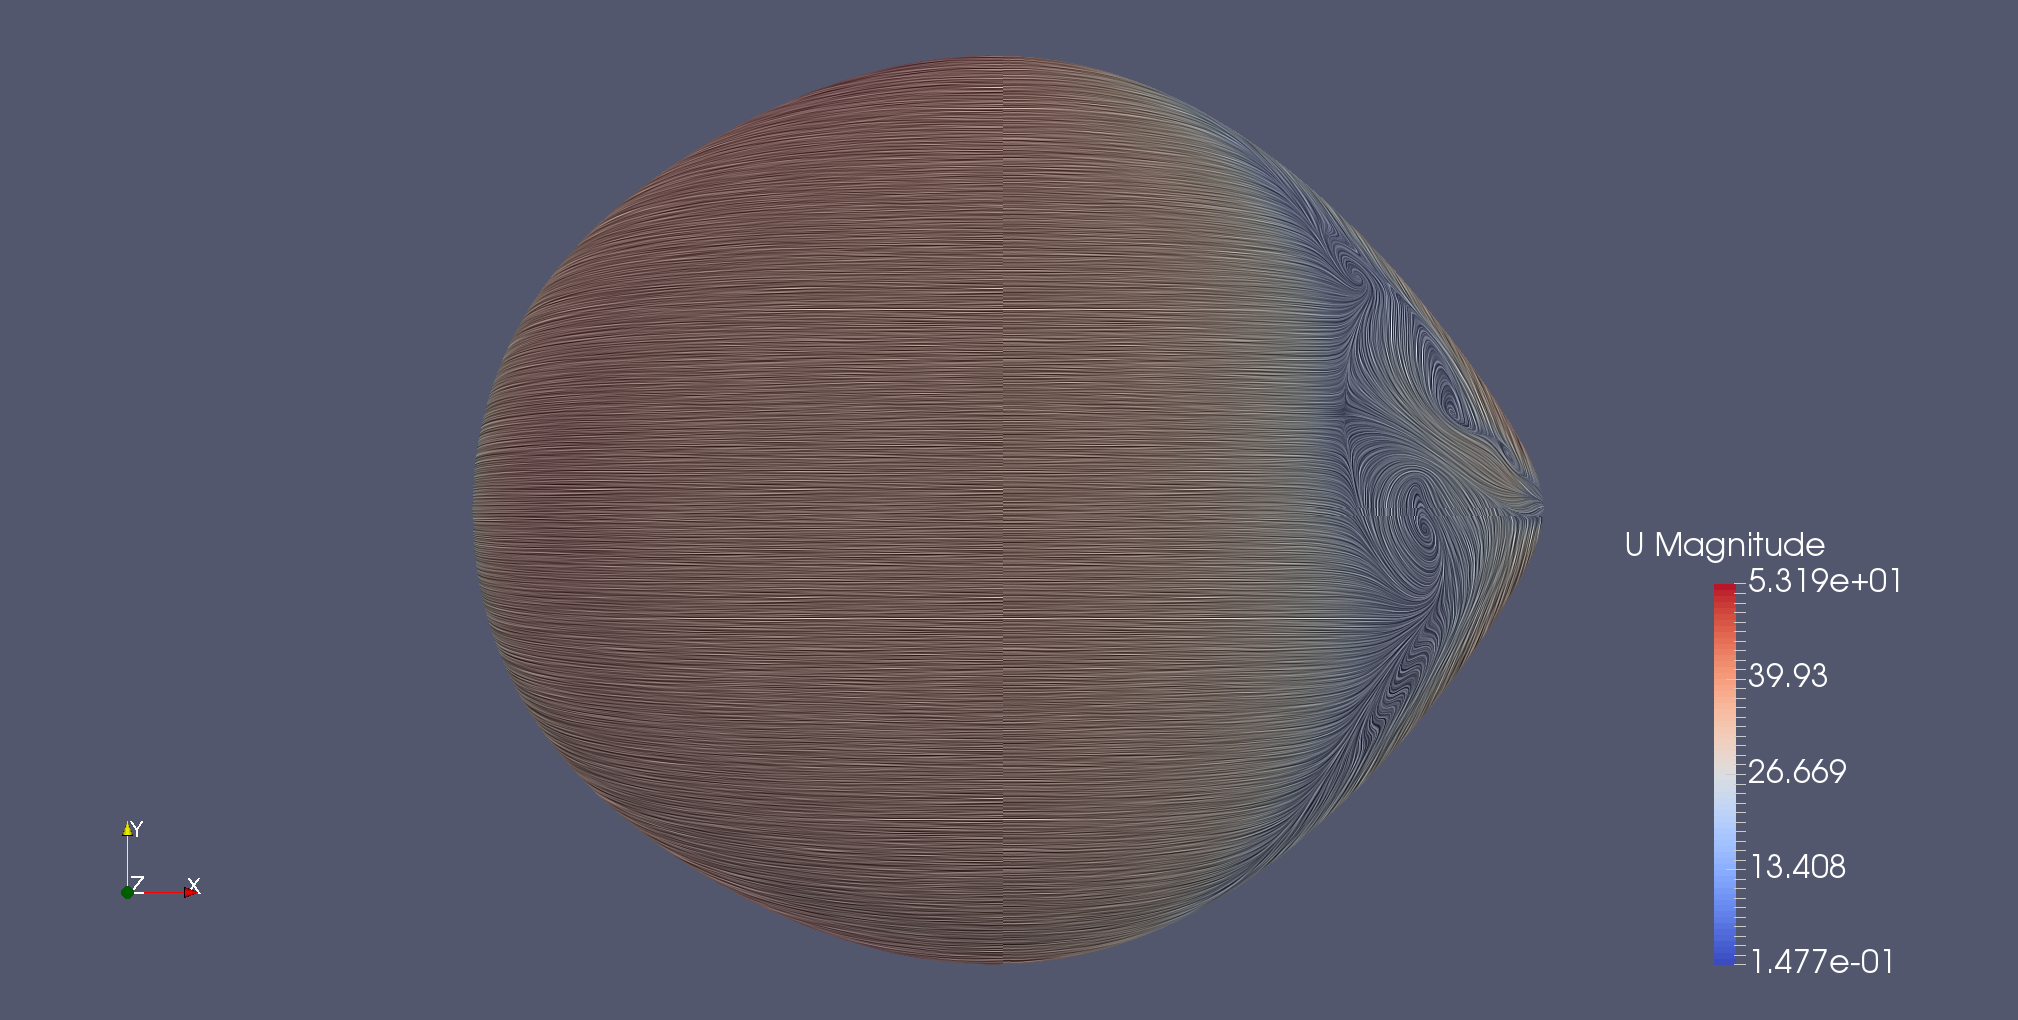
\includegraphics[width=300 pt]{rnd/streamlines_45.png}
	\caption{Surface streamlines on the body with high pressure drag}
	\label{high drag body} %      only if needed
\end{figure}

Thus there is flow separation phenomenon involved in the CFD analysis of non-axisymmetric shapes. To capture this non-linear we need large number of design points to be considered. Also, to get more accurate results un-steady flow simulations are to be carried out and the time average of drag values has to be taken to while fitting the model.

\section{Sub-optimal results obtained}
Since it is not possible to get completely optimal results with the existing model, we can obtain sub-optimal results using the following method.
To explain the concept of sub-optimal results, consider modified Himmelblau function discussed in section \ref{Modified Himmelblau function}. From Figure \ref{fig:Root Mean Square Error with Design Points considered}, we can infer that we need at least 150 design points to get develop a surrogate model which mimics actual Himmelblau function. But instead of 150 points, lets take only 20 points and construct a Kriging surrogate model and find the optimal point. It is already known that the optimal points is  (-3.7793,-3.2872). If we couple the genetic algorithm optimizer with surrogate model developed using only 20 points, we get the following results.
\begin{table}[H]
	\centering
	\caption{Results obtained for 20 design points}
	\label{Results obtained for 20 design points}
	%\begin{ruledtabular}
	\begin{tabular}{llll}
		\hline \hline
		& X & Y & Function value \\ \hline
		Actual Function & -3.7793 &-3.2832 &1.3278e-13 \\
		Surrogate model & -3.2205 &-2.9549 & -6.3131 \\ \hline
		\% error & 14.79 & 10.00 & 6.3131 \\
		\hline \hline
	\end{tabular}
	%	\end{ruledtabular}
\end{table}
From the above table we may see that if the number of design points used to train the model are low and if this model is coupled with optimizer, we end up getting sub-optimal solution with some percentage error. In the same way, if we couple genetic algorithm optimizer with the surrogate model obtained, we will arrive at sub-optimal results. The results obtained are shown in Table \ref{Optimal solution obtained}.


\begin{table}[H]
	\centering
	\caption{sub-optimal solution obtained for miminum $ C_{DV} $}
	\label{sub-optimal solution obtained}
	%\begin{ruledtabular}
	\begin{tabular}{lc}
		\hline \hline
		Design Parameters & Optimal value for minimum $ C_{DV} $    \\ \hline \hline
		
		$ Point\ of\ Max.\ Dia., m$ & 0.44960      \\  
		$ Nose\ Radius, r _{o} $ & 0.38316    \\
		$ Tail\ Radius, r _{1} $ & 0.23247     \\  
		$ Prismatic\ Coeff., C _{p }$ & 0.60598 \\
		$ Fineness\ Ratio, \frac{l}{d} $ &4.28392 \\
		$Scaling\ in\ Y\ direction,\ scale\_y$ &1.50423 \\ \hline \hline
		
		$ Kriging C_{DV} $ & \\
		$ OpenFOAM\textsuperscript{\textregistered} C_{DV} $ & \\
		$ \% Error $ & \\
		\hline \hline
	\end{tabular}
	%	\end{ruledtabular}
\end{table}

\section{Multi-disciplinary shape optimisation}
Two disciplines namely aerodynamics and structures which involves the calculation of aerodynamic drag ($ C_{DV} $) and von-mises ($ \sigma _{v} $) stress are considered for shape optimisation of airship profile. The aim is to have lowest possible aerodynamic drag and Von-Mises stress. To acieve this, we develop a composite objective function minimising which, both $ C_{DV} $ and $ \sigma _{v} $ are minimised simultaneously.
The objective function is defined as
\begin{equation}
F_{comp} = \frac{1}{2}\bigg( \frac{C_{DV}}{C_{DV,ref}} + \dfrac{\sigma _{v}}{\sigma _{v,ref}} \bigg)
\end{equation}

Where, $C_{DV,ref} , \sigma _{v,ref}  $ are the values of these parameters corresponding to the reference shape.  The values obtained in Table \ref{sub-optimal solution obtained} and \ref{Optimal solution obtained for mimimum sigma_v} are taken as reference values for $C_{DV,ref}$ and $\sigma _{v,ref}  $ respectively. The composite objective function now becomes:
\begin{equation}
F_{comp} = 0.5*( C_{DV} + \sigma _{v})
\end{equation}
